\documentclass[12pt]{scrartcl}

\usepackage[utf8]{inputenc}
\usepackage[T1]{fontenc}
\usepackage{lmodern}
\usepackage{graphicx}
\usepackage[pdftex,hyperref,dvipsnames]{xcolor}
\usepackage{listings}
\usepackage[a4paper,lmargin={2cm},rmargin={2cm},tmargin={3.5cm},bmargin = {2.5cm},headheight = {4cm}]{geometry}
\usepackage{amsmath,amssymb,amstext,amsthm}
% \usepackage[lined,algonl,boxed]{algorithm2e} 
\usepackage{algpseudocode}
\usepackage{tikz}
\usepackage{pgfplots}
\usepackage{hyperref}
\usepackage{url}
\usepackage{tcolorbox}
\usepackage{float}
\usepackage[inline]{enumitem}
\usepackage[headsepline]{scrlayer-scrpage} 

\usetikzlibrary{automata,positioning}

\usepgfplotslibrary{external}
%\tikzexternalize
\pgfplotsset{width=10cm,compat=1.9}
\pgfplotsset{every axis/.style={
    axis line style = thick,
    grid = both,
    tick pos = left,
    tick align = outside,
    tick style = {thick,black},
    fill = blue,
	line width = 2pt,
}}

\lstset{
  basicstyle=\ttfamily\small,
  numbers=left,
  numberstyle=\tiny,
  stepnumber=1,
  numbersep=8pt,
  frame=single,
  breaklines=true,
  columns=fullflexible
}

\lstset{
  language=C,
  basicstyle=\ttfamily\small,
  keywordstyle=\color{blue},
  commentstyle=\color{gray},
  stringstyle=\color{green!60!black},
  numbers=left,
  numberstyle=\tiny,
  stepnumber=1,
  numbersep=8pt,
  frame=single,
  breaklines=true,
  columns=fullflexible
}

\renewcommand{\theenumi}{(\alph{enumi})}
\renewcommand{\labelenumi}{\text{\theenumi}}
\renewcommand{\labelenumii}{(\roman{enumii})} 

\ohead{Weiting Wang (3855168)\\
       Nico Strohbach (3546914)\\
       Jan Theil (3794698)}

\ihead{Reinforcement Learning}

\newcounter{exnum}
\newcommand{\exercise}[1]{\section*{Problem \theexnum\stepcounter{exnum}: #1}}

\begin{document}

\setcounter{exnum}{1}
\exercise{Random Walk}

The TD(0) update is defined as: $V(S_t) = V(S_t) + \alpha [R_{t + 1} + \gamma V(S_{t + 1}) - V(S_t)]$.
In the plot one can see that all $V(S_t)$ have been initialized with $0.5$.
For $\gamma \neq 1$ every step from $S_t \neq A$  would change $V(S_t)$ by a small fraction $\implies$ In this case we must have started from $A$.
If $\gamma = 1$ the walk from $C \to \ldots \to A$ would not change any $V(S_t)$ values. When $A$ is reached in this case, the following argument also applies:
During this episode we must have reached / started from state $A$ and then transistioned to the terminal state $T_0$ left to it: $A \to T_0$.
With $\alpha = 0.1$ and the convention $V(S_{terminal}) = 0.0$ this would update
\begin{align*}
  V(A) &= V(A) + \alpha [R_{t + 1} + \gamma V(T_0) - V(A)] \\
       &= 0.5 + \alpha [0.0 + 0.0 - 0.5] \\
       &= 0.5 - \alpha 0.5 \\
       &= 0.45
\end{align*}

Since a terminal state has been reached, the evaluation of this episode is finished and with the same argumentation as above
obviously no other estimates are changed during the process.

\exercise{Sarsa and Q-learning on the FrozenLake}

\begin{enumerate}
  \item For the code, please see \textit{ex05-td.py}. We have implemented \texttt{sarsa()} with an
        $\epsilon$-greedy policy.
        \begin{figure}[H]
          \centering
          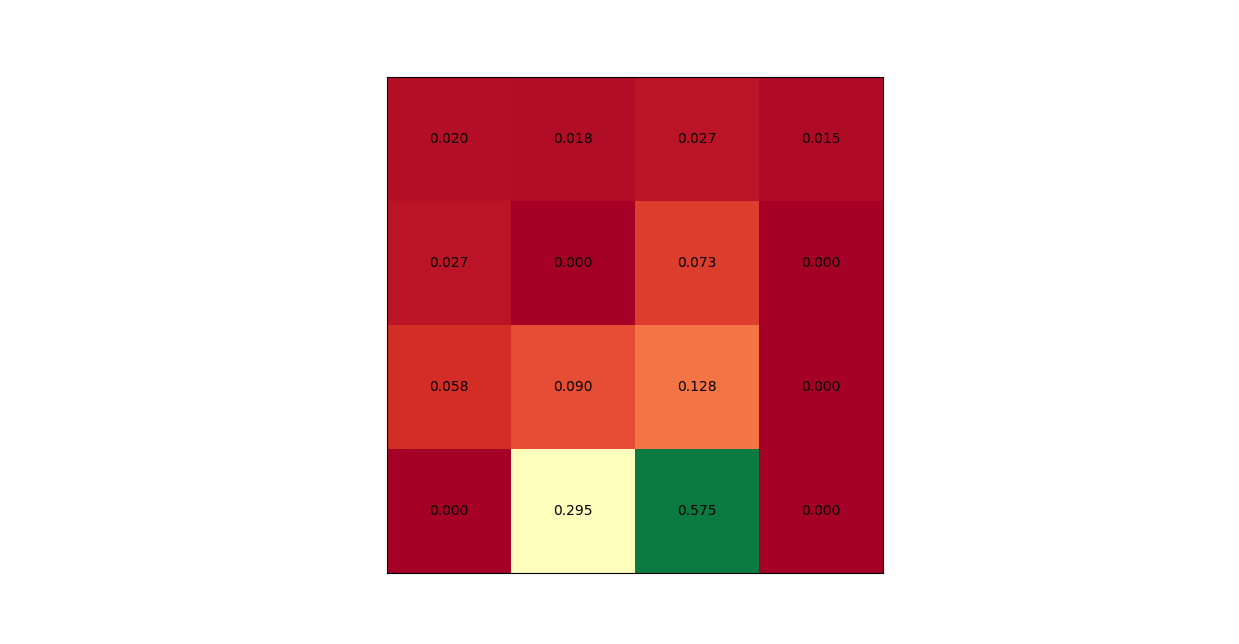
\includegraphics[width=\textwidth]{sarsa_v.png}
          \caption{State-value function}
          \label{fig:sarsa_v}

        \end{figure}
        \begin{figure}[H]
          \centering
          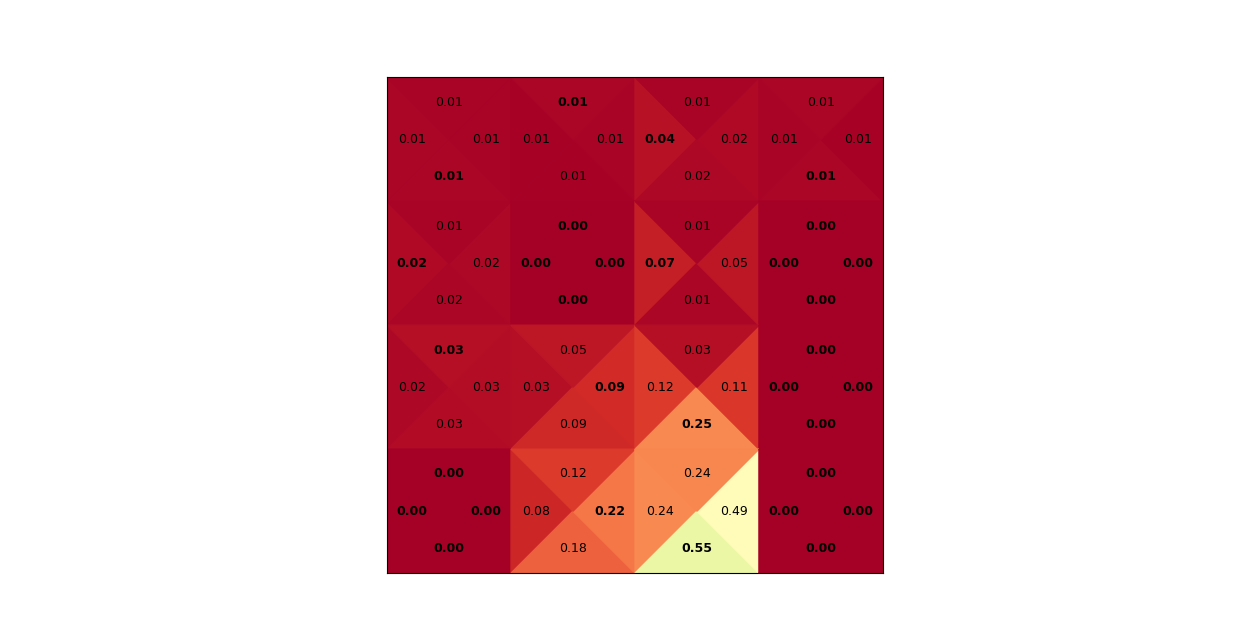
\includegraphics[width=\textwidth]{sarsa_q.png}
          \caption{Action-Value function}
          \label{fig:sarsa_q}
        \end{figure}

        \[
        \begin{array}{cccc}
        \leftarrow & \uparrow & \leftarrow & \uparrow \\
        \leftarrow & H & \rightarrow & H \\
        \uparrow & \downarrow & \leftarrow & H \\
        H & \rightarrow & \downarrow & G
        \end{array}
        \]
        \[
        \text{Policy}
        \]
\end{enumerate}


\end{document}